\section{Overview: High-level components and their interaction}
\label{s:overview}%

\section{Component view}
\label{s:component-view}%

\section{Deployment view}
\label{s:deployment-view}%

\newpage

\section{Runtime view}
\label{s:runtime-view}%
This section contains the sequence diagrams of the most important operations of the system. The diagrams include the component that we have already described in the previous section and the external components that are involved in the operations.

\subsubsection*{User Registration}
\label{ss:registration_diagram}%
When a user wants to register to the system, he/she has to fill in the registration form and submit it. The difference between a ST and an ED is in the information passed with \textit{UserInfo} object, where the ED has to insert also the information about the institution he/she works for.

The whole process is mainly handled by the \textit{Authentication Manager} component, that interact with the \textit{Data Manager} component to validate the information and insert the new user into the DBMS.

The system will check if the information inserted are valid and if the user is not already registered. This check is done internally from CKB and if the information are valid and the user is not already registered, the system will insert it into the DBMS and sends an email to the user with a link to confirm the registration, using the \textit{Notification Manager} component. The user will click on the link and the \textit{Authentication Manager} will confirm the registration.

If the information inserted are not valid, the user is already registered or the confirmation link is expired, the system will send an error message to the user.

\begin{figure}[H]
  \centering
  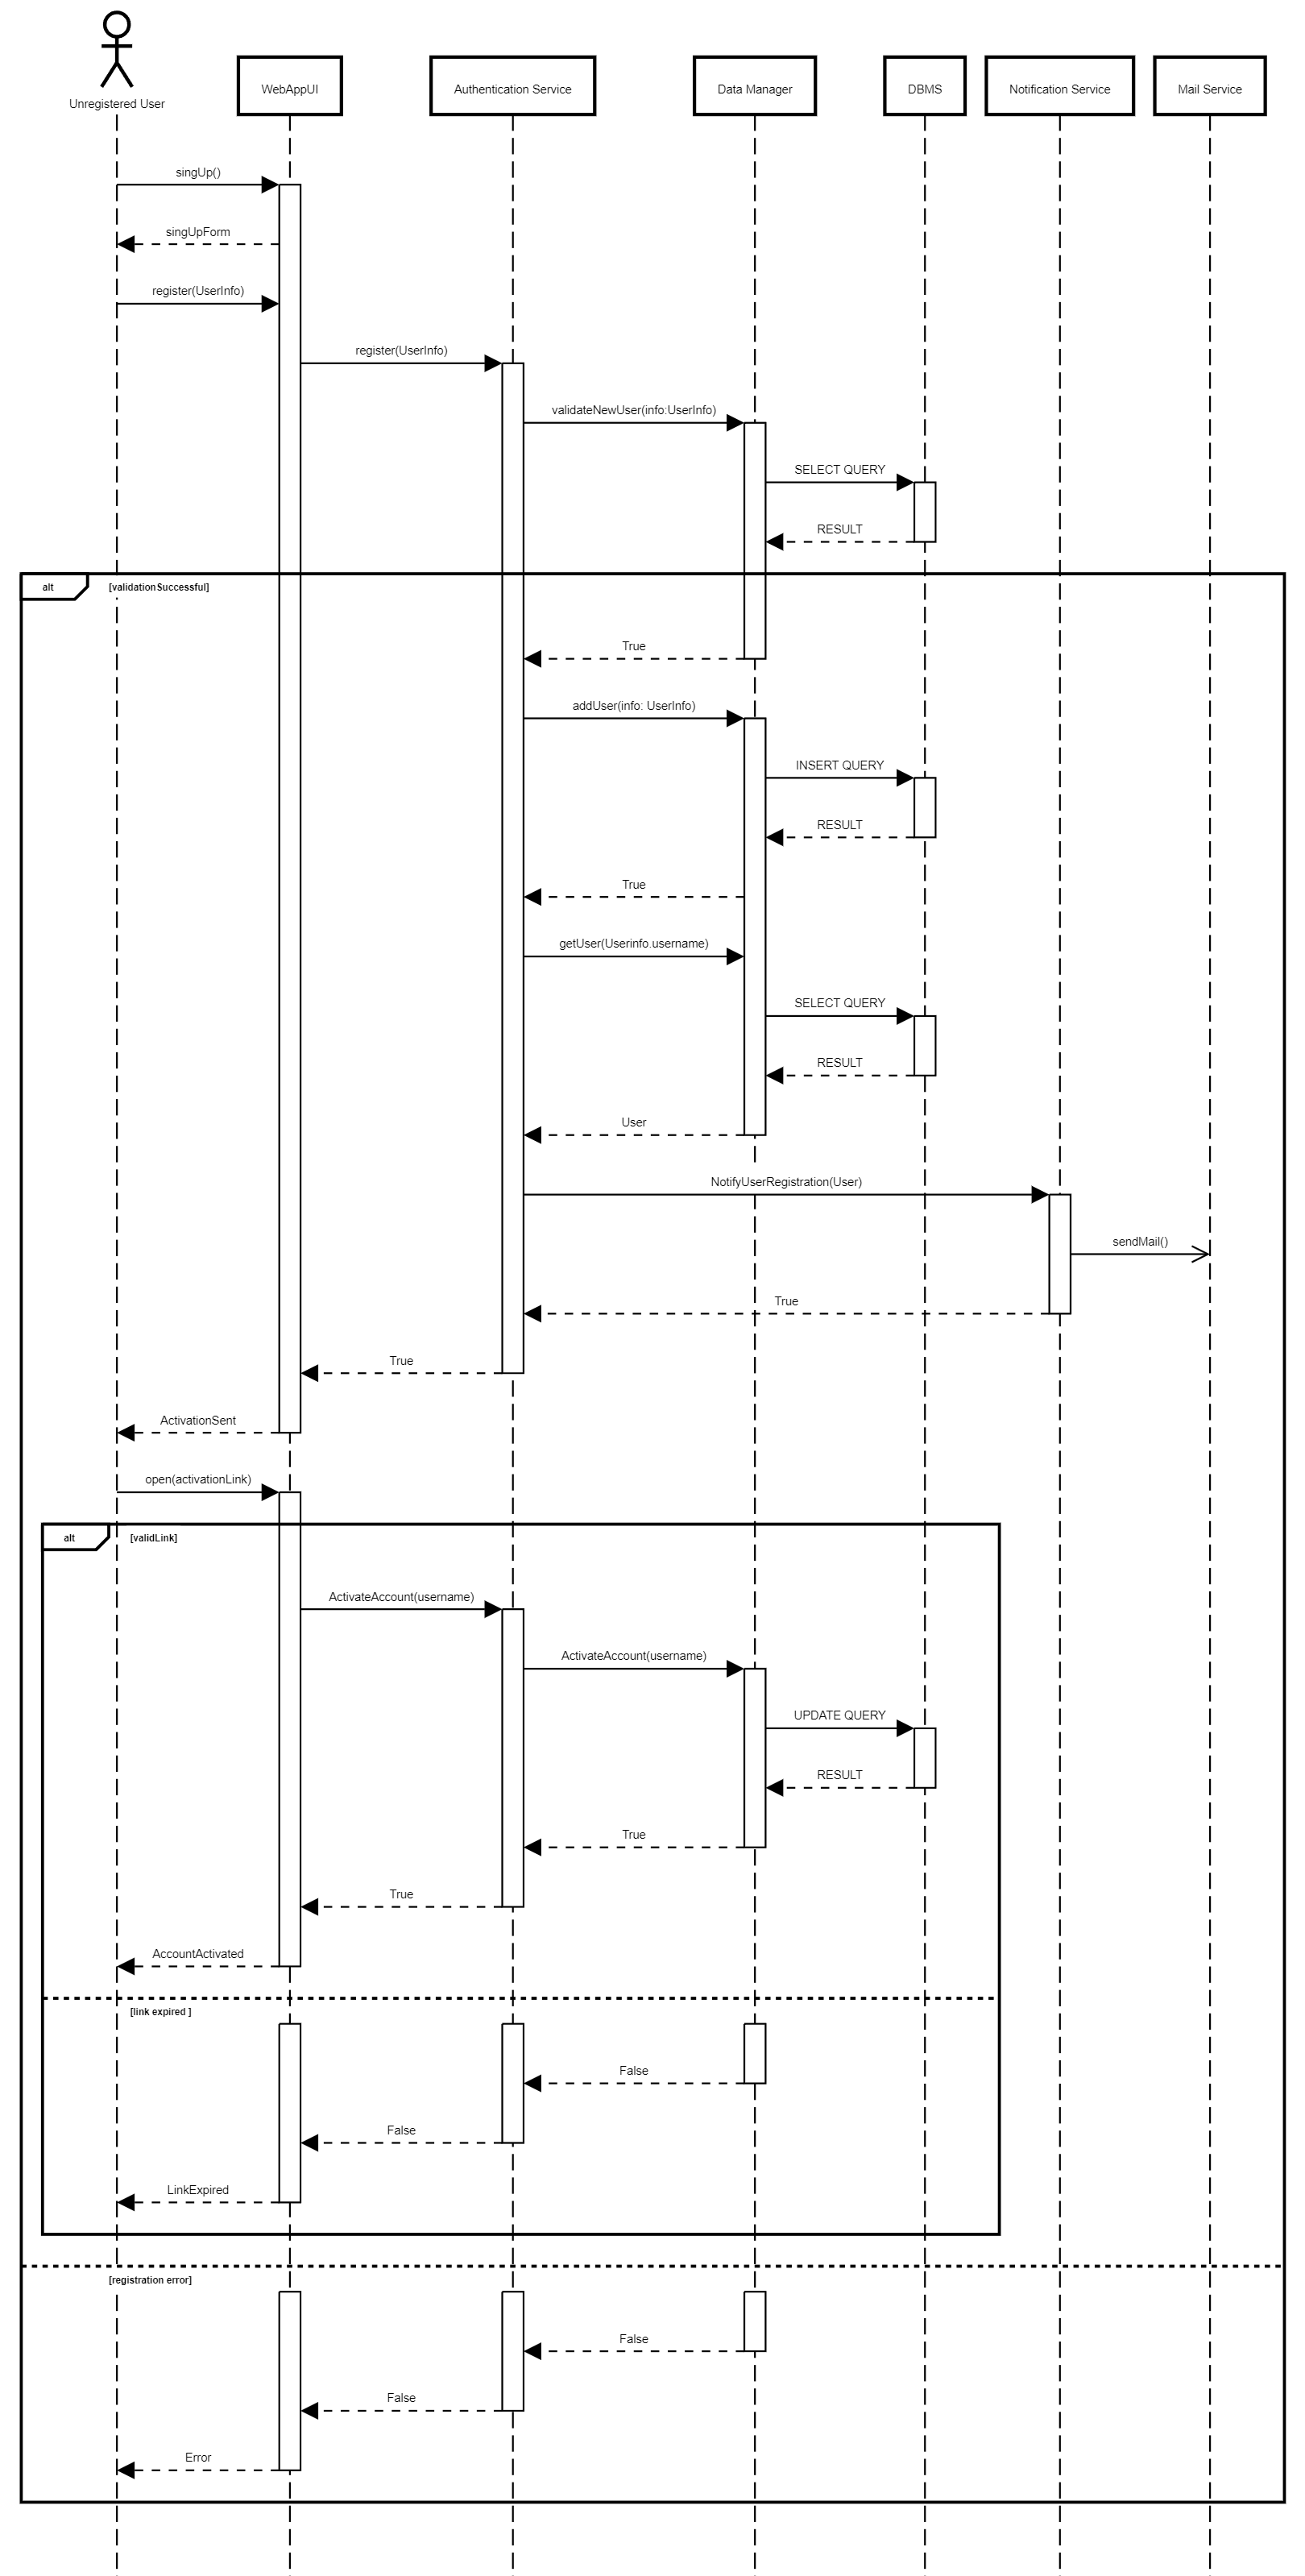
\includegraphics[width=\textwidth,height=\textheight, keepaspectratio]{SequenceDiagrams/01-UserRegistration.png}
  \caption{Registration sequence diagram}
  \label{fig:registratio_diagramn}
\end{figure}

\subsubsection*{User Login}
\label{ss:login_diagram}%
When a user wants to login to the system, he/she has to fill in the login form and submit it. This process is equal for both the ST and the ED. As the User Registration, the whole process is handled by the \textit{Authentication Manager} component, that interact with the \textit{Data Manager} component to validate the information. Once the user is logged in, the \textit{Authentication Manager} will generate a token for the user, send it to the client and the user can finally access the dashboard.

If the login information are not valid, the system will show an error message to the user.

\begin{figure}[H]
  \centering
  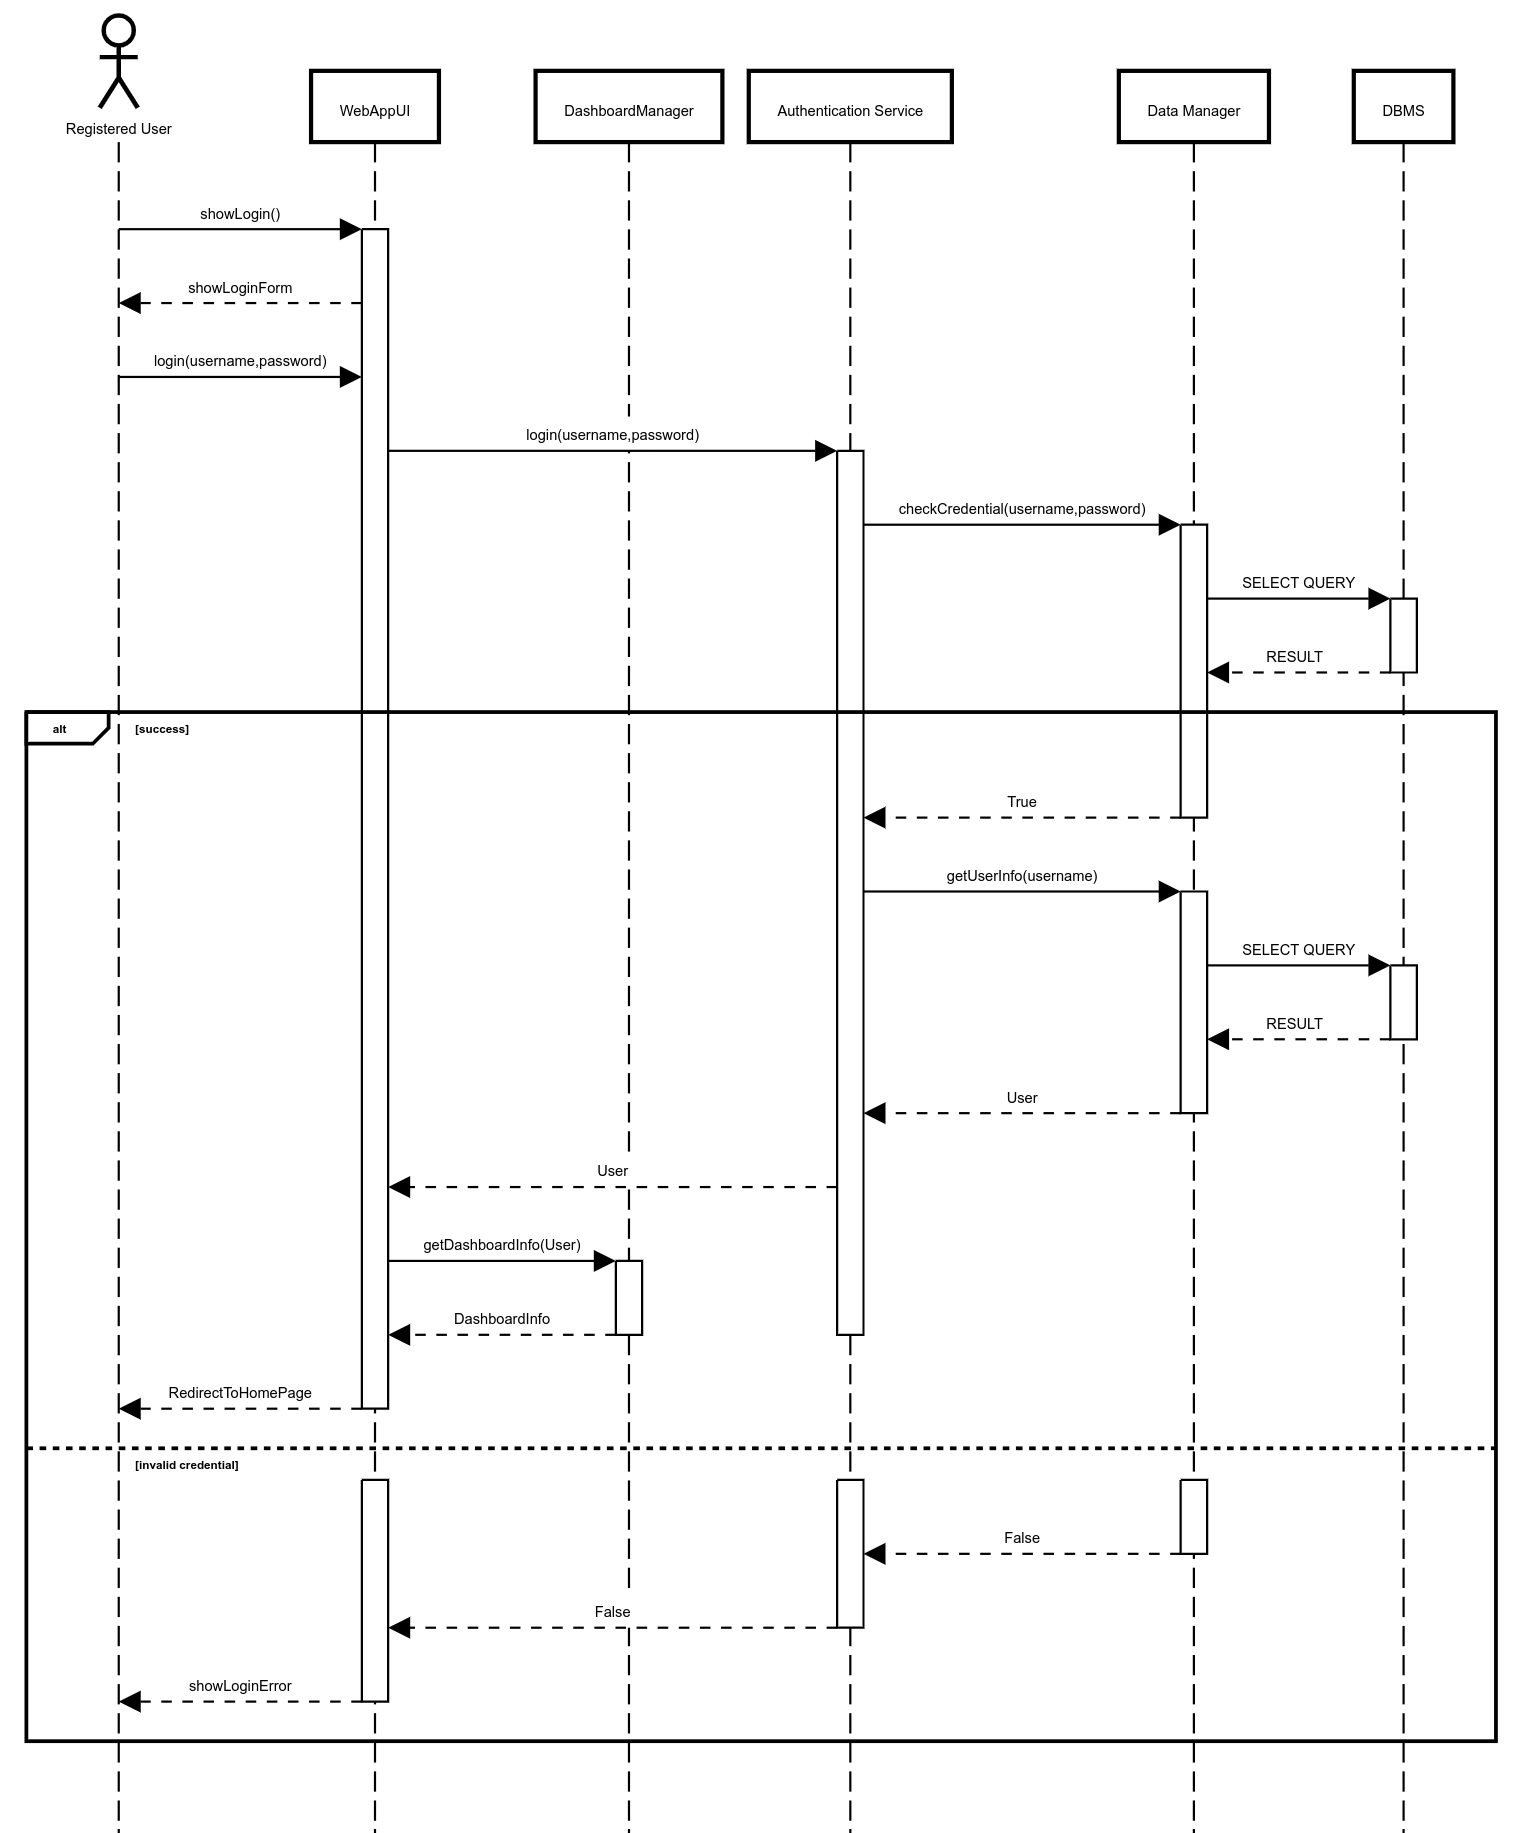
\includegraphics[width=\textwidth,height=0.7\textheight, keepaspectratio]{SequenceDiagrams/02-UserLogin.png}
  \caption{Login sequence diagram}
  \label{fig:login_diagramn}
\end{figure}

\subsubsection*{ED Creates Competition}
\label{ss:create_competition_diagram}
Here is shown how a competition is created by an ED. The ED has to fill in the form with the information about the competition and submit it. The \textit{Competition Manager} component will check if the name is available and if so the competition will be created and inserted into the DBMS using the \textit{Data Manager} component, otherwise a new name will be requested. The system will then returns the competition and will be shown the competition page.

\begin{figure}[H]
  \centering
  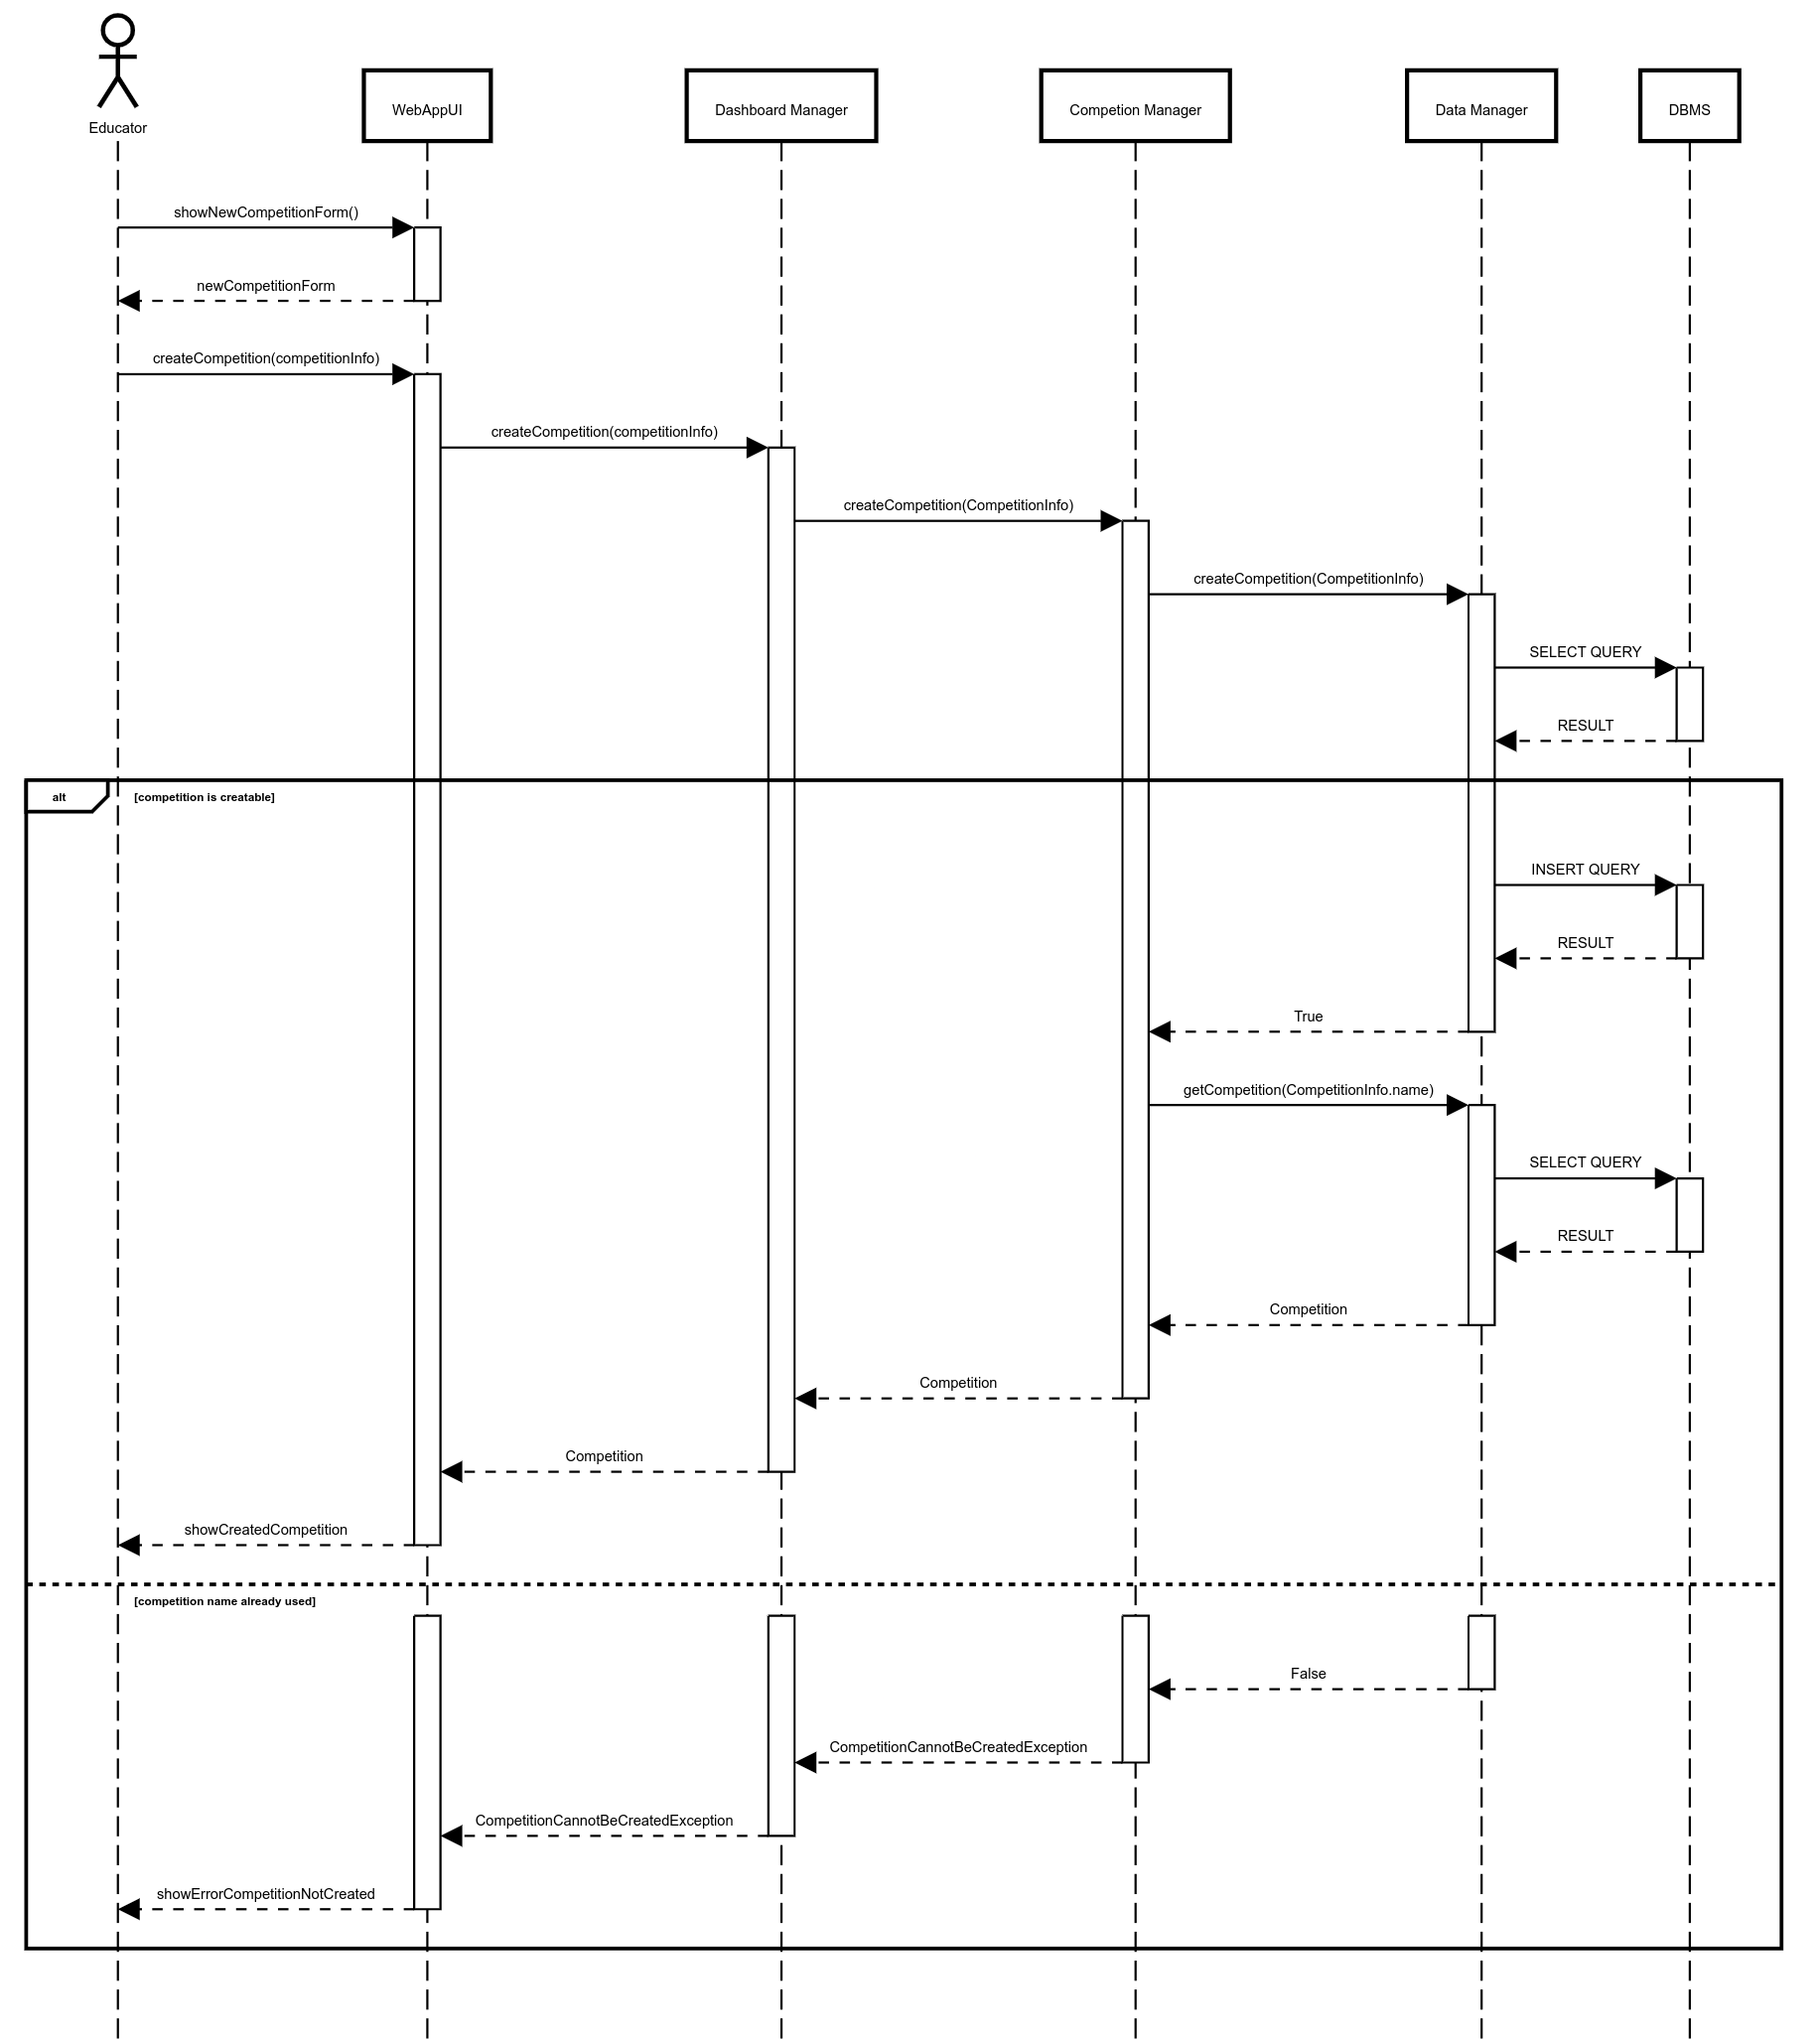
\includegraphics[width=\textwidth,height=0.74\textheight, keepaspectratio]{SequenceDiagrams/04-EducatorCreatesCompetition.png}
  \caption{Create competition sequence diagram}
  \label{fig:create_competition_diagramn}
\end{figure}

\subsubsection*{ST Joins Competition}
\label{ss:join_competition_diagram}
The ST firstly visualize all the available competitions in the platform, then he/she can choose one of them and join it. The \textit{Competition Manager} component will handle both the search of the available competitions and the insertion into the DBMS using the \textit{Data Manager} component. The system will then show a success message to the user.

\begin{figure}[H]
  \centering
  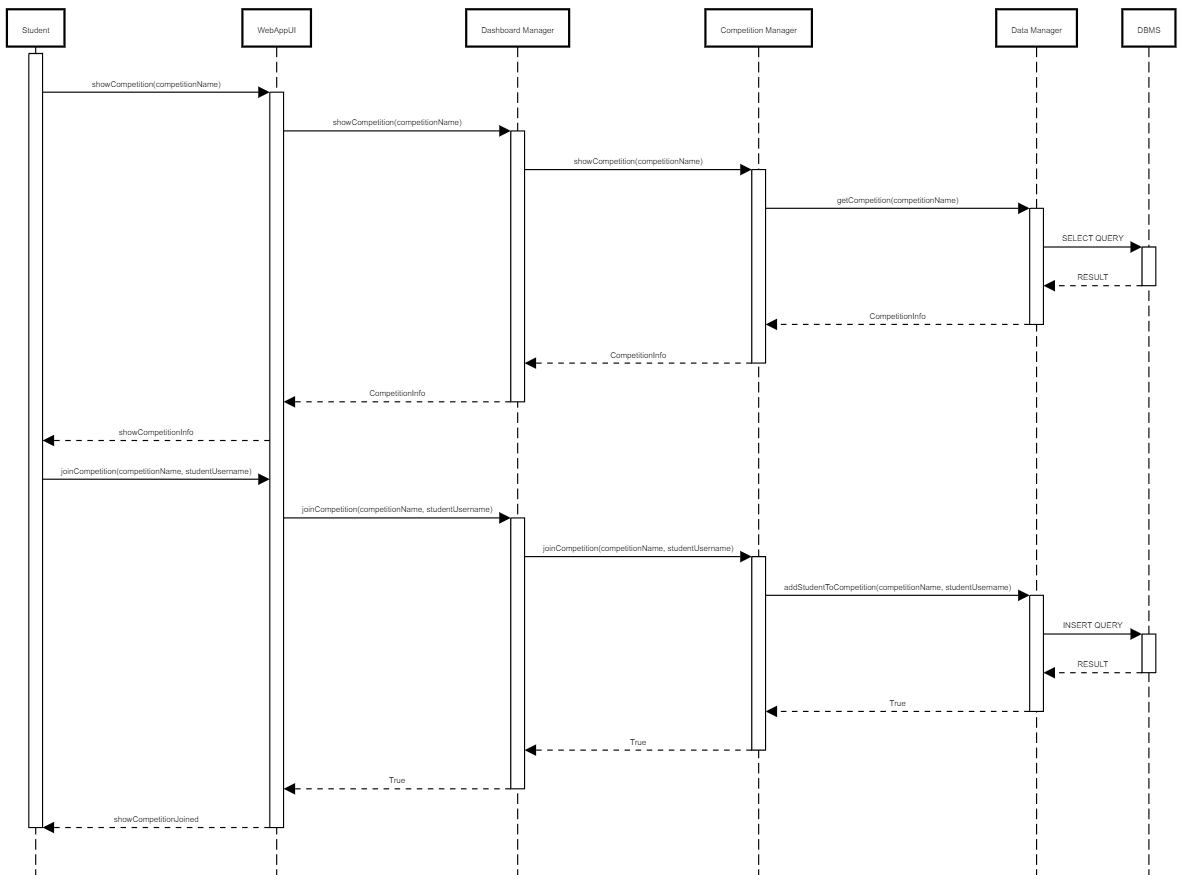
\includegraphics[width=\textwidth,height=\textheight, keepaspectratio]{SequenceDiagrams/05-StudentJoinCompetition.png}
  \caption{Join competition sequence diagram}
  \label{fig:join_competition_diagramn}
\end{figure}

\subsection*{ED Creates Battle}
\label{ss:create_battle_diagram}
When a ED wants to create a battle, he/she needs to be in a competition page that he/she manages. The interaction is divided in two parts: the first one is where the ED inserts the general information about the battle, the name is then validated by the \textit{Battle Manager} component and if it is valid the system will show the second part of the form where the ED can insert the information about the automatic evaluation and static analysis. The \textit{Battle Manager} component will check if the information are valid and if so the battle will be created and inserted into the DBMS using the \textit{Data Manager} component.

If the battle is successfully created, the system will send a notification, through the \textit{Notification Manager} to all the ST enrolled in the competition where the battle has been created.

\begin{figure}[H]
  \centering
  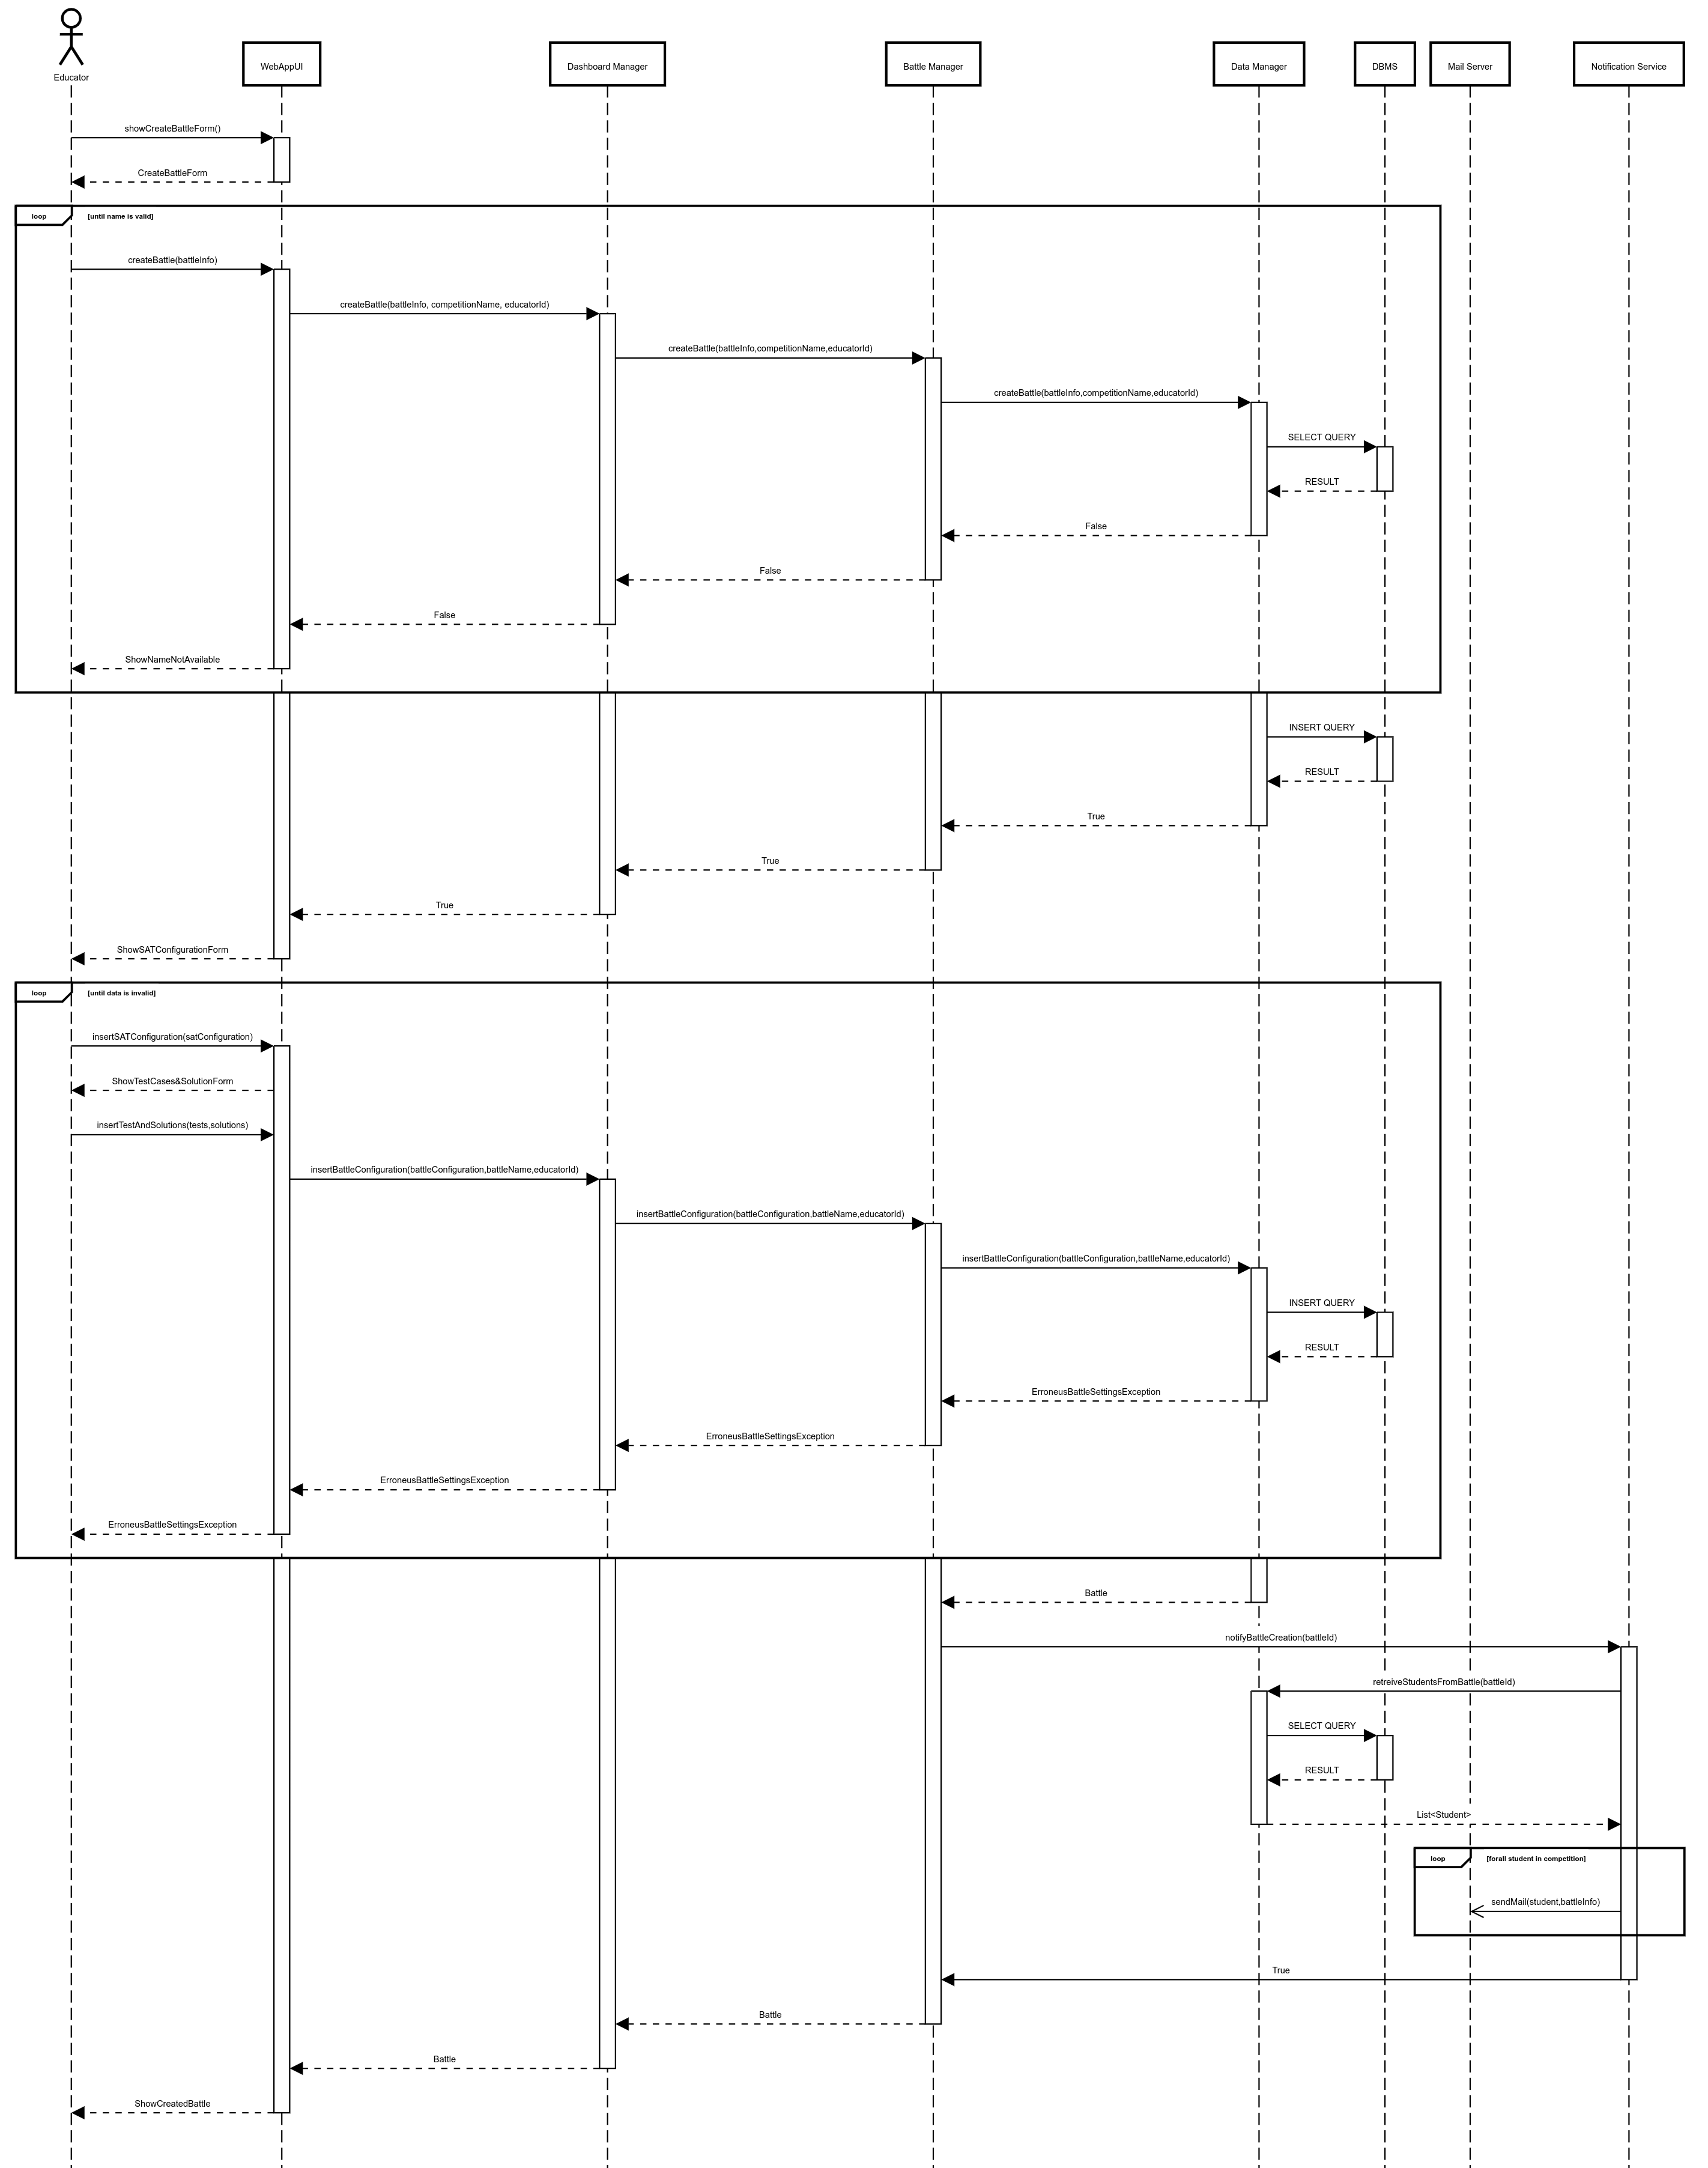
\includegraphics[width=\textwidth,height=0.83\textheight, keepaspectratio]{SequenceDiagrams/06-EducatorCreatesBattle.png}
  \caption{Create battle sequence diagram}
  \label{fig:create_battle_diagramn}
\end{figure}

\section{Component interfaces}
\label{s:component-interfaces}%

\section{Selected architectural styles and patterns}
\label{s:selected-architectural-styles-and-patterns}%

\section{Other design decisions}
\label{s:other-design-decisions}%
